\Chapter{Étude de plasmas magnétisé}
\chaptermark{Étude de plasmas magnétisé}
\begin{refsection}

	\section{Plasma de bord des tokamaks}
		 
	\section{Barrière magnétique : PEGASES}
		\begin{figure}[htbp]
\centering
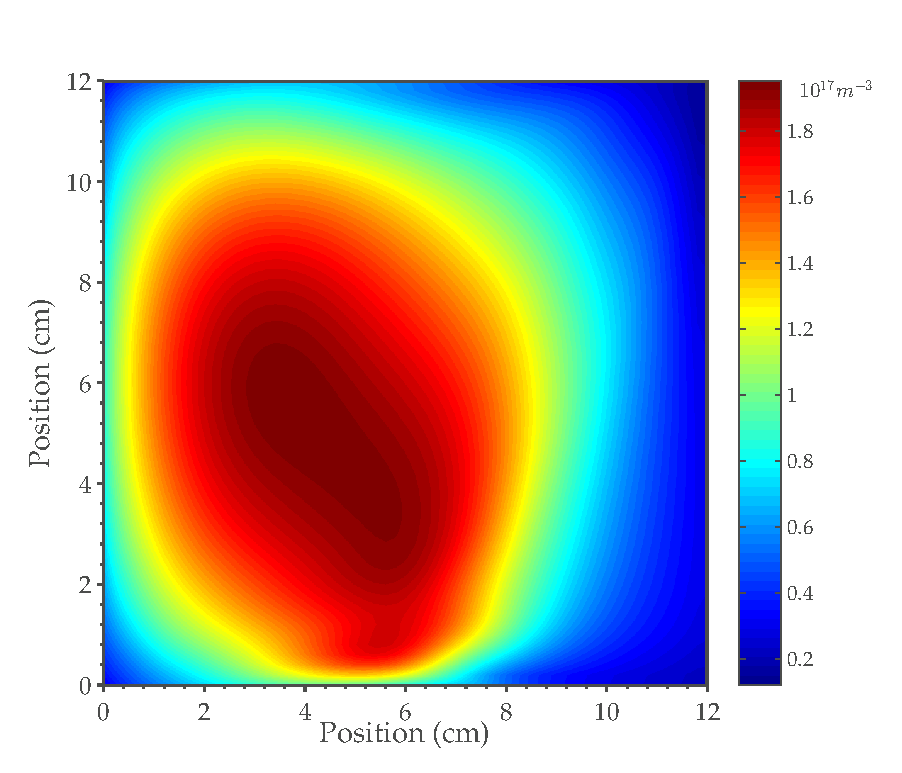
\includegraphics[height=0.7\textwidth,width=0.9\textwidth]{figures/pegasescarteDensite.eps}{\caption{Carte
de densité dans le propulseur.
}\label{4-pegasesDensite}}
\end{figure}
	\section{Colonne de plasma magnétisé : CYBELE}
	\includegraphics[width=\textwidth]{figures/pegasesCarteCourant.eps}

		
	
%\bibliographystyle{apalike}
%\bibliography{biblio}
\end{refsection}
